\documentclass[12pt]{article}
\usepackage[margin=1in]{geometry}
\usepackage{graphicx}
\usepackage{amsmath, amssymb}
\usepackage{booktabs}
\usepackage{float}
\usepackage{caption}
\captionsetup[figure]{labelfont=bf, font=it}
\usepackage{hyperref}
\usepackage{setspace}
\usepackage{siunitx}

\hypersetup{colorlinks=true, linkcolor=blue, urlcolor=blue, citecolor=blue}

\title{\textbf{\LARGE Electric Field Mapping} \\ \large Dipole Configuration - Lab 5}
\author{Sean Rockwitz, Abhiraj Singh}
\date{\textit{19 February, 2026} \\ \textit{PHYS 180, Dr.\ Ray Sameshima} \\ \textit{New York Institute of Technology}}

\begin{document}

% ============================================================
% TITLE PAGE
% ============================================================
\begin{titlepage}
    \centering
    \vspace*{1.2cm}
    {\Huge \textbf{Electric Field Mapping} \par}
    \vspace{0.3cm}
    {\Large Dipole Configuration - Lab 5 \par}
    \vspace{0.6cm}
    \rule{\textwidth}{0.4pt}
    \vspace{0.5cm}

    {\large Sean Rockwitz, Abhiraj Singh \par}
    \vspace{0.2cm}
    {\large \textit{19 February, 2026} \par}
    {\large \textit{PHYS 180, Dr.\ Ray Sameshima} \par}
    {\large \textit{New York Institute of Technology} \par}

    \vspace{0.8cm}

    \begin{figure}[H]
        \centering
        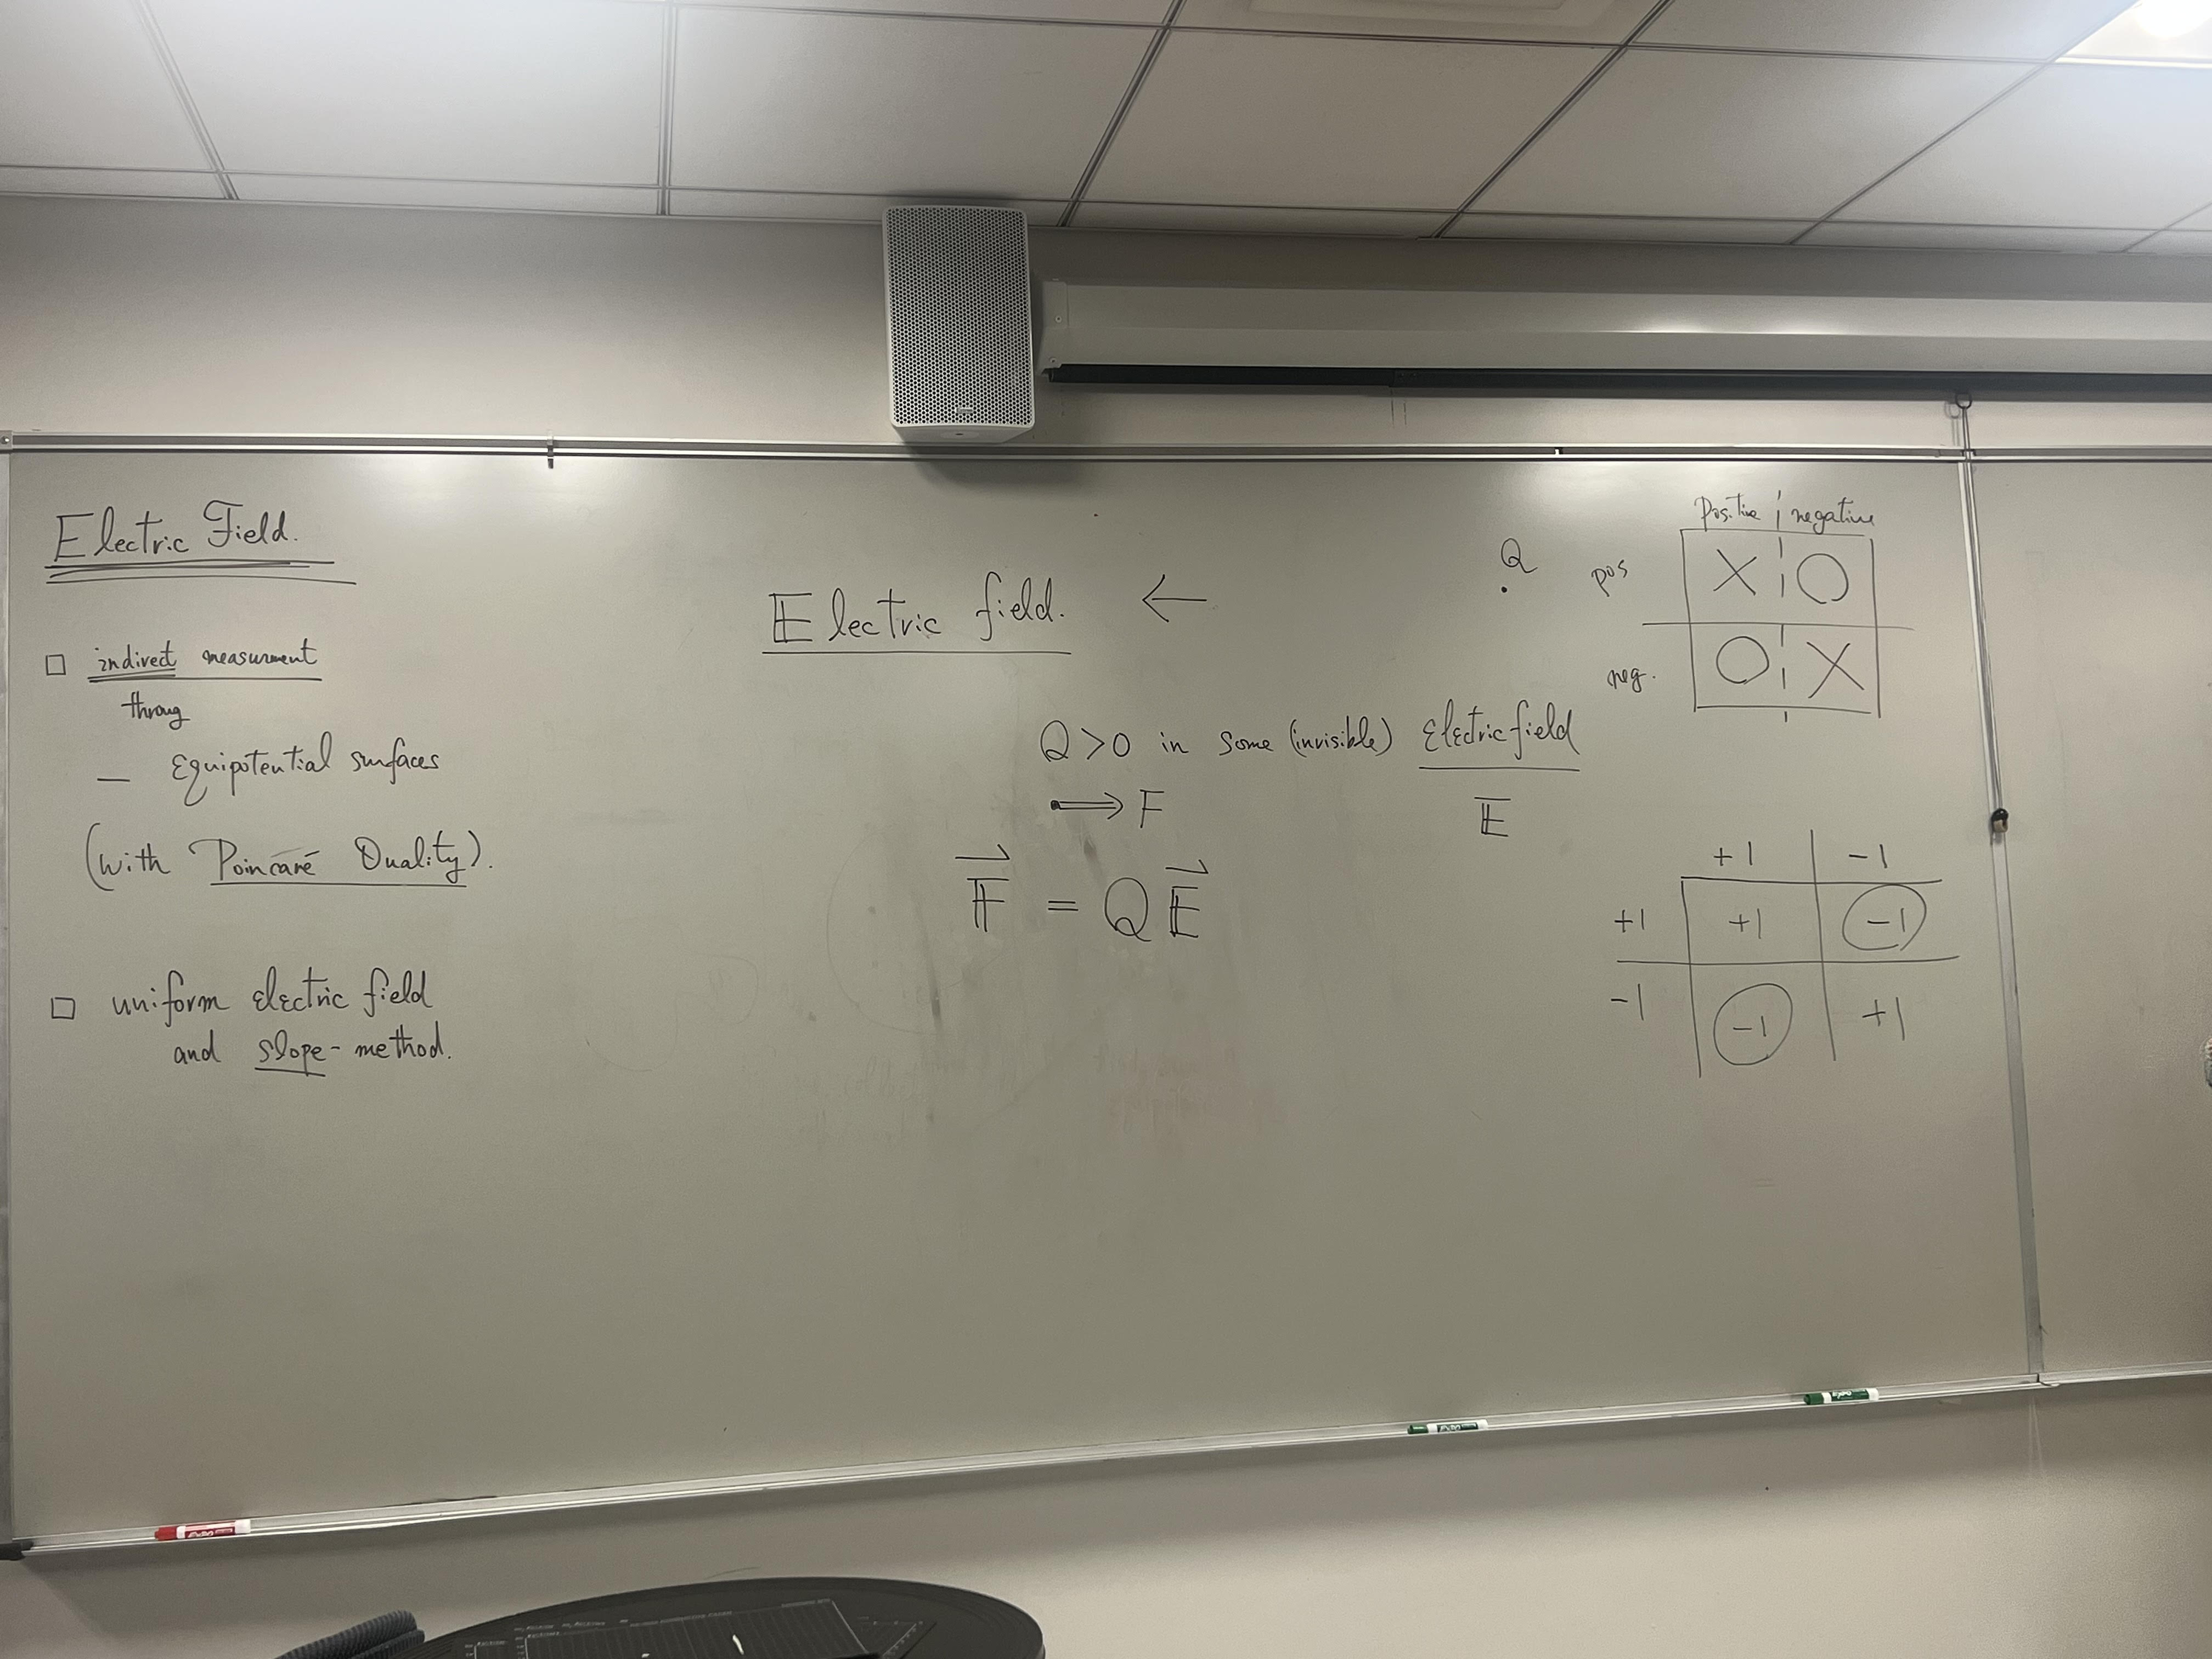
\includegraphics[width=0.7\textwidth]{lecture_notes.jpeg}
        \caption*{\textbf{Figure 1.} \textit{Lecture notes on electric field theory and the indirect measurement approach through equipotential surfaces.}}
    \end{figure}

\end{titlepage}

% ---- 1. LEARNING OBJECTIVES ----
\section{Learning Objectives}

The goal of this lab was to map out the equipotential lines of a dipole on two-dimensional conductive paper. We applied a fixed voltage across two point electrodes and used a multimeter to find positions on the paper where the potential difference between a reference point and the probe was zero. Tracing these zero-voltage positions gives us the equipotential curves, and since electric field lines are always perpendicular to equipotential surfaces, the curves tell us what the field looks like without ever measuring it directly.

I (Sean) recorded the data points and built the visualization, while Abhiraj handled the probes, sweeping the measurement probe across the paper and dialing in on the zero-voltage positions.

% ---- 2. MAIN CONCEPTS ----
\section{Main Concepts and Formulae}

The electric field $\vec{E}$ is one of the most important quantities in electrostatics, but you can't measure it directly. What you can do is measure the electric potential $V$ at various points and work backwards using

\begin{equation}
    \vec{E} = -\nabla V
\end{equation}

The field points in the direction of steepest potential decrease and is perpendicular to equipotential surfaces everywhere. So if you can map out where the potential is constant, you know the shape of the field.

\subsection{Force and Field}

A positive test charge $Q > 0$ sitting in an external electric field $\vec{E}$ feels a force

\begin{equation}
    \vec{F} = Q\vec{E}
\end{equation}

This is the whole idea behind the indirect measurement approach from lecture (Figure~1): we can't see the field itself, but we can observe what it does to charges. Mapping the potential landscape is an equivalent way to characterize the field.

\subsection{Dipole Potential on Conductive Paper}

On two-dimensional conductive paper, the potential from a single point electrode falls off logarithmically with distance (unlike the $1/r$ behavior in three dimensions). When you have two electrodes, one positive and one negative, the total potential at any point $(x, y)$ is just the superposition of the two:

\begin{equation}
    V(x, y) = C \ln\!\left(\frac{r_-}{r_+}\right)
\end{equation}

Here $r_-$ and $r_+$ are the distances to the negative and positive electrodes, and $C$ is a constant that depends on the applied voltage. Along the perpendicular bisector of the two electrodes, $r_- = r_+$, so $V = 0$. That bisector becomes the axis of symmetry for the entire equipotential map.

\subsection{Symmetry}

The dipole has two symmetries that saved us a lot of work:

\begin{itemize}
    \item \textbf{Left-right symmetry:} The equipotential pattern is symmetric about the perpendicular bisector of the two electrodes (the axis of symmetry at $x = 14$ in our case). We only had to measure the left half and could reflect it to get the right.
    \item \textbf{Top-bottom symmetry:} The pattern is also symmetric about the line connecting the electrodes ($y = 10$). So the $x$-value at $y = 12$ should match the one at $y = 8$, the value at $y = 14$ should match $y = 6$, and so on.
\end{itemize}

% ---- 3. PROCEDURE ----
\section{Procedure}

The setup was pretty simple. Two thumbtack electrodes were pressed into the PASCO PK-9025 conductive paper at positions $(10, 10)$ and $(18, 10)$, giving a separation of 8~cm and putting the axis of symmetry at $x = 14$. A DC power supply held a constant 2.4~V across the electrodes the whole time. The conductive paper has a centimeter grid printed right on it, which made reading off coordinates straightforward.

\begin{figure}[H]
    \centering
    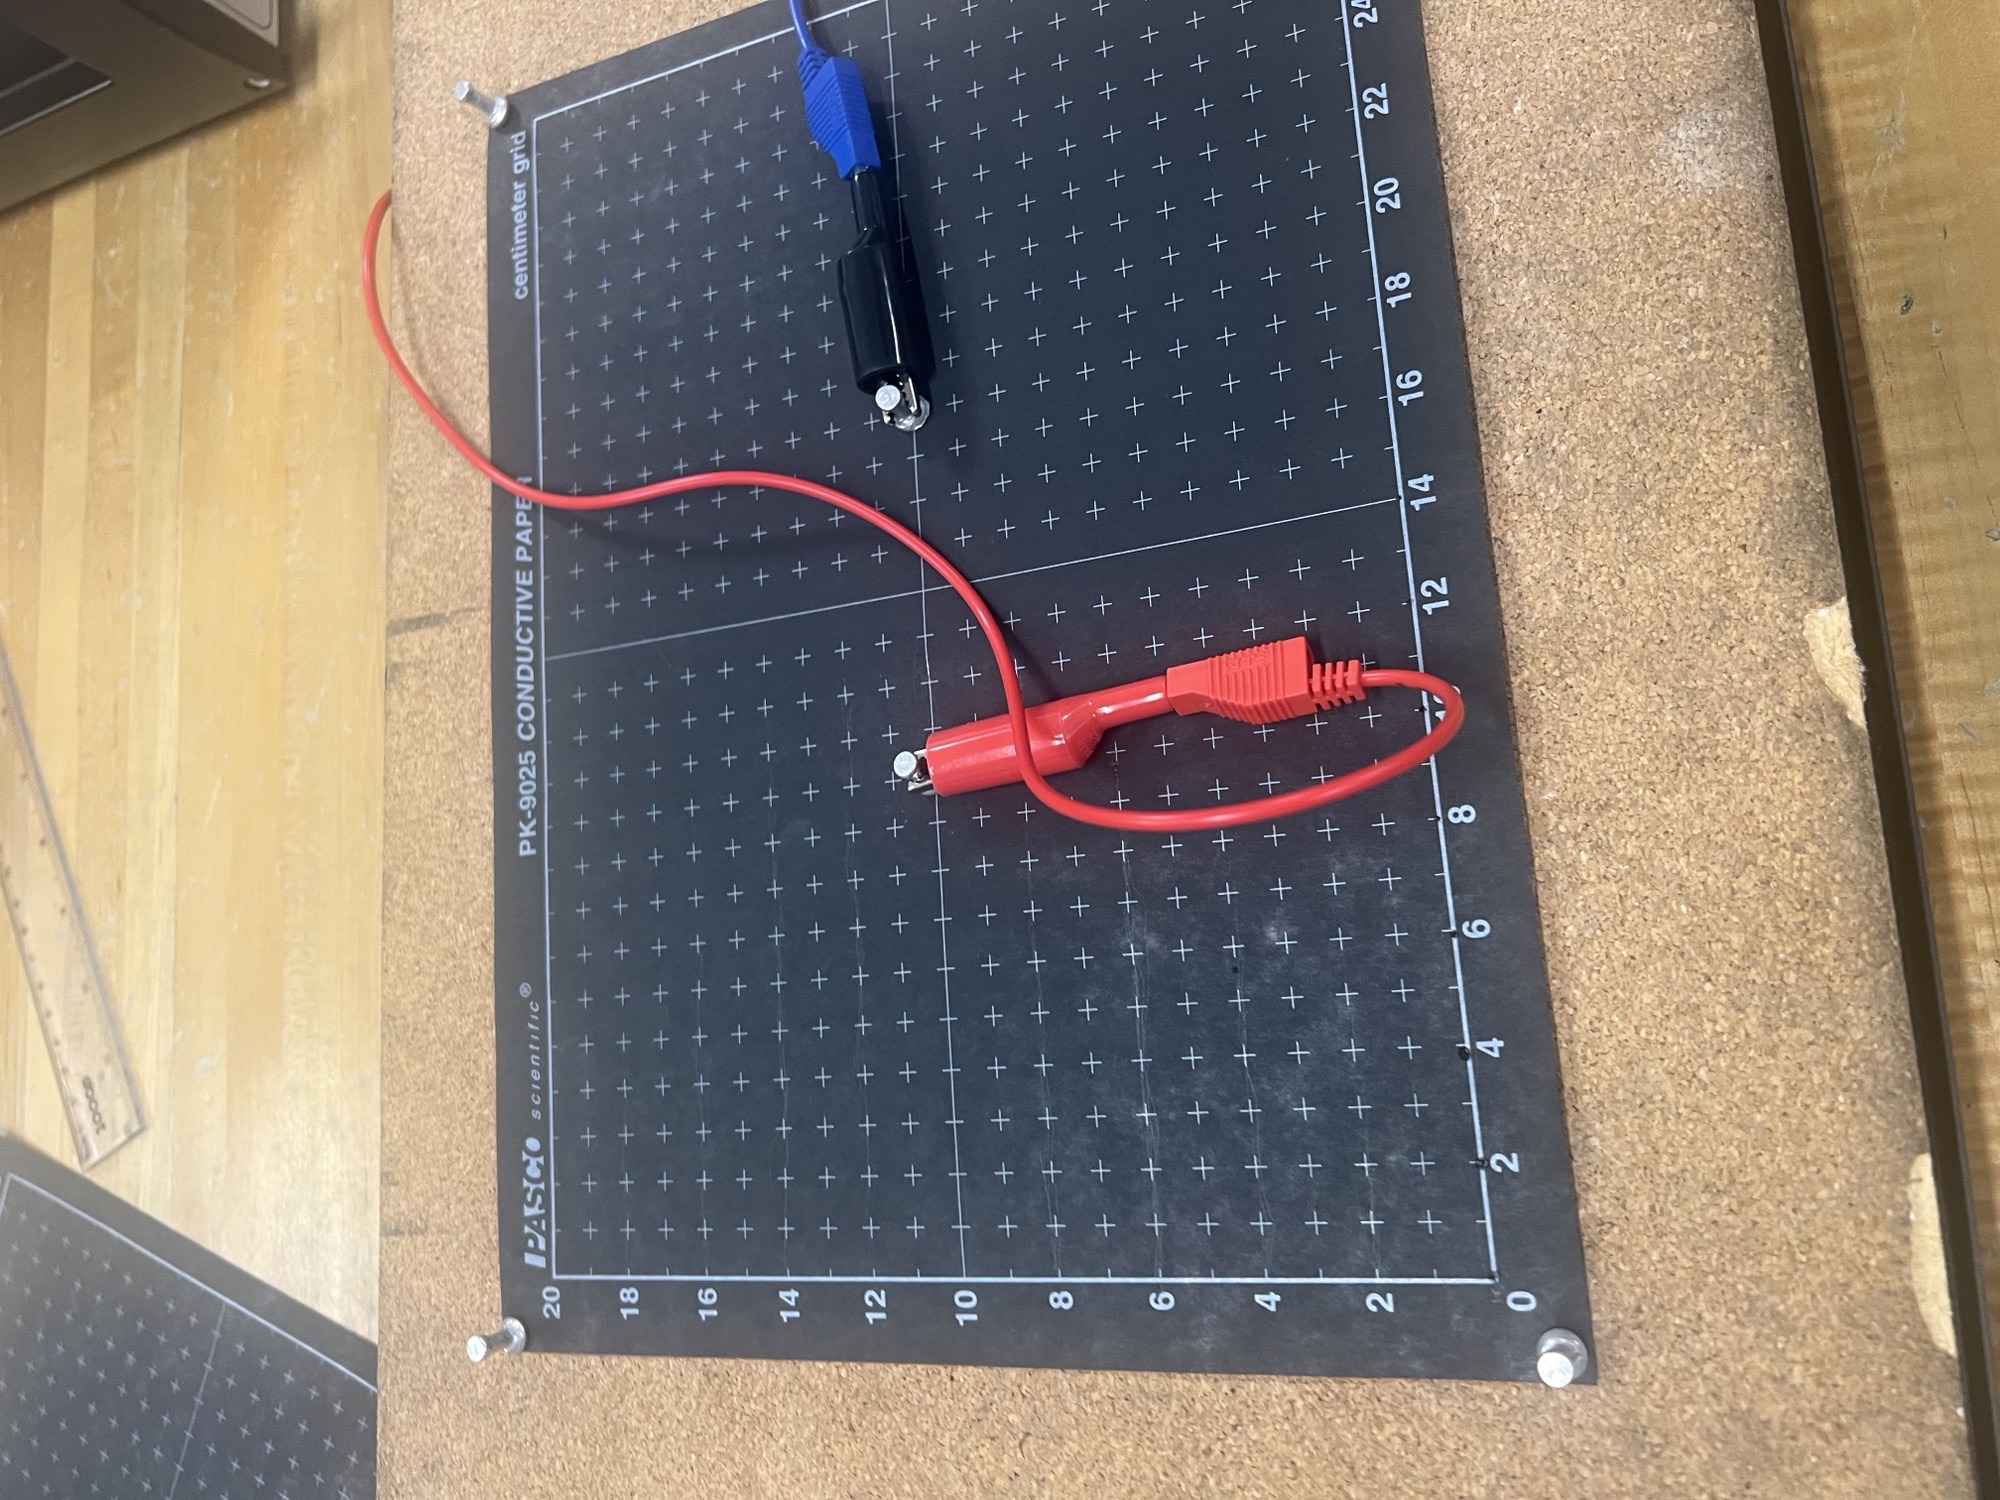
\includegraphics[width=0.55\textwidth]{conductive_paper.jpeg}
    \caption{PASCO PK-9025 conductive paper with electrodes connected. The centimeter grid is visible, and the two thumbtack electrodes are connected via alligator clips to the power supply.}
    \label{fig:paper}
\end{figure}

\begin{figure}[H]
    \centering
    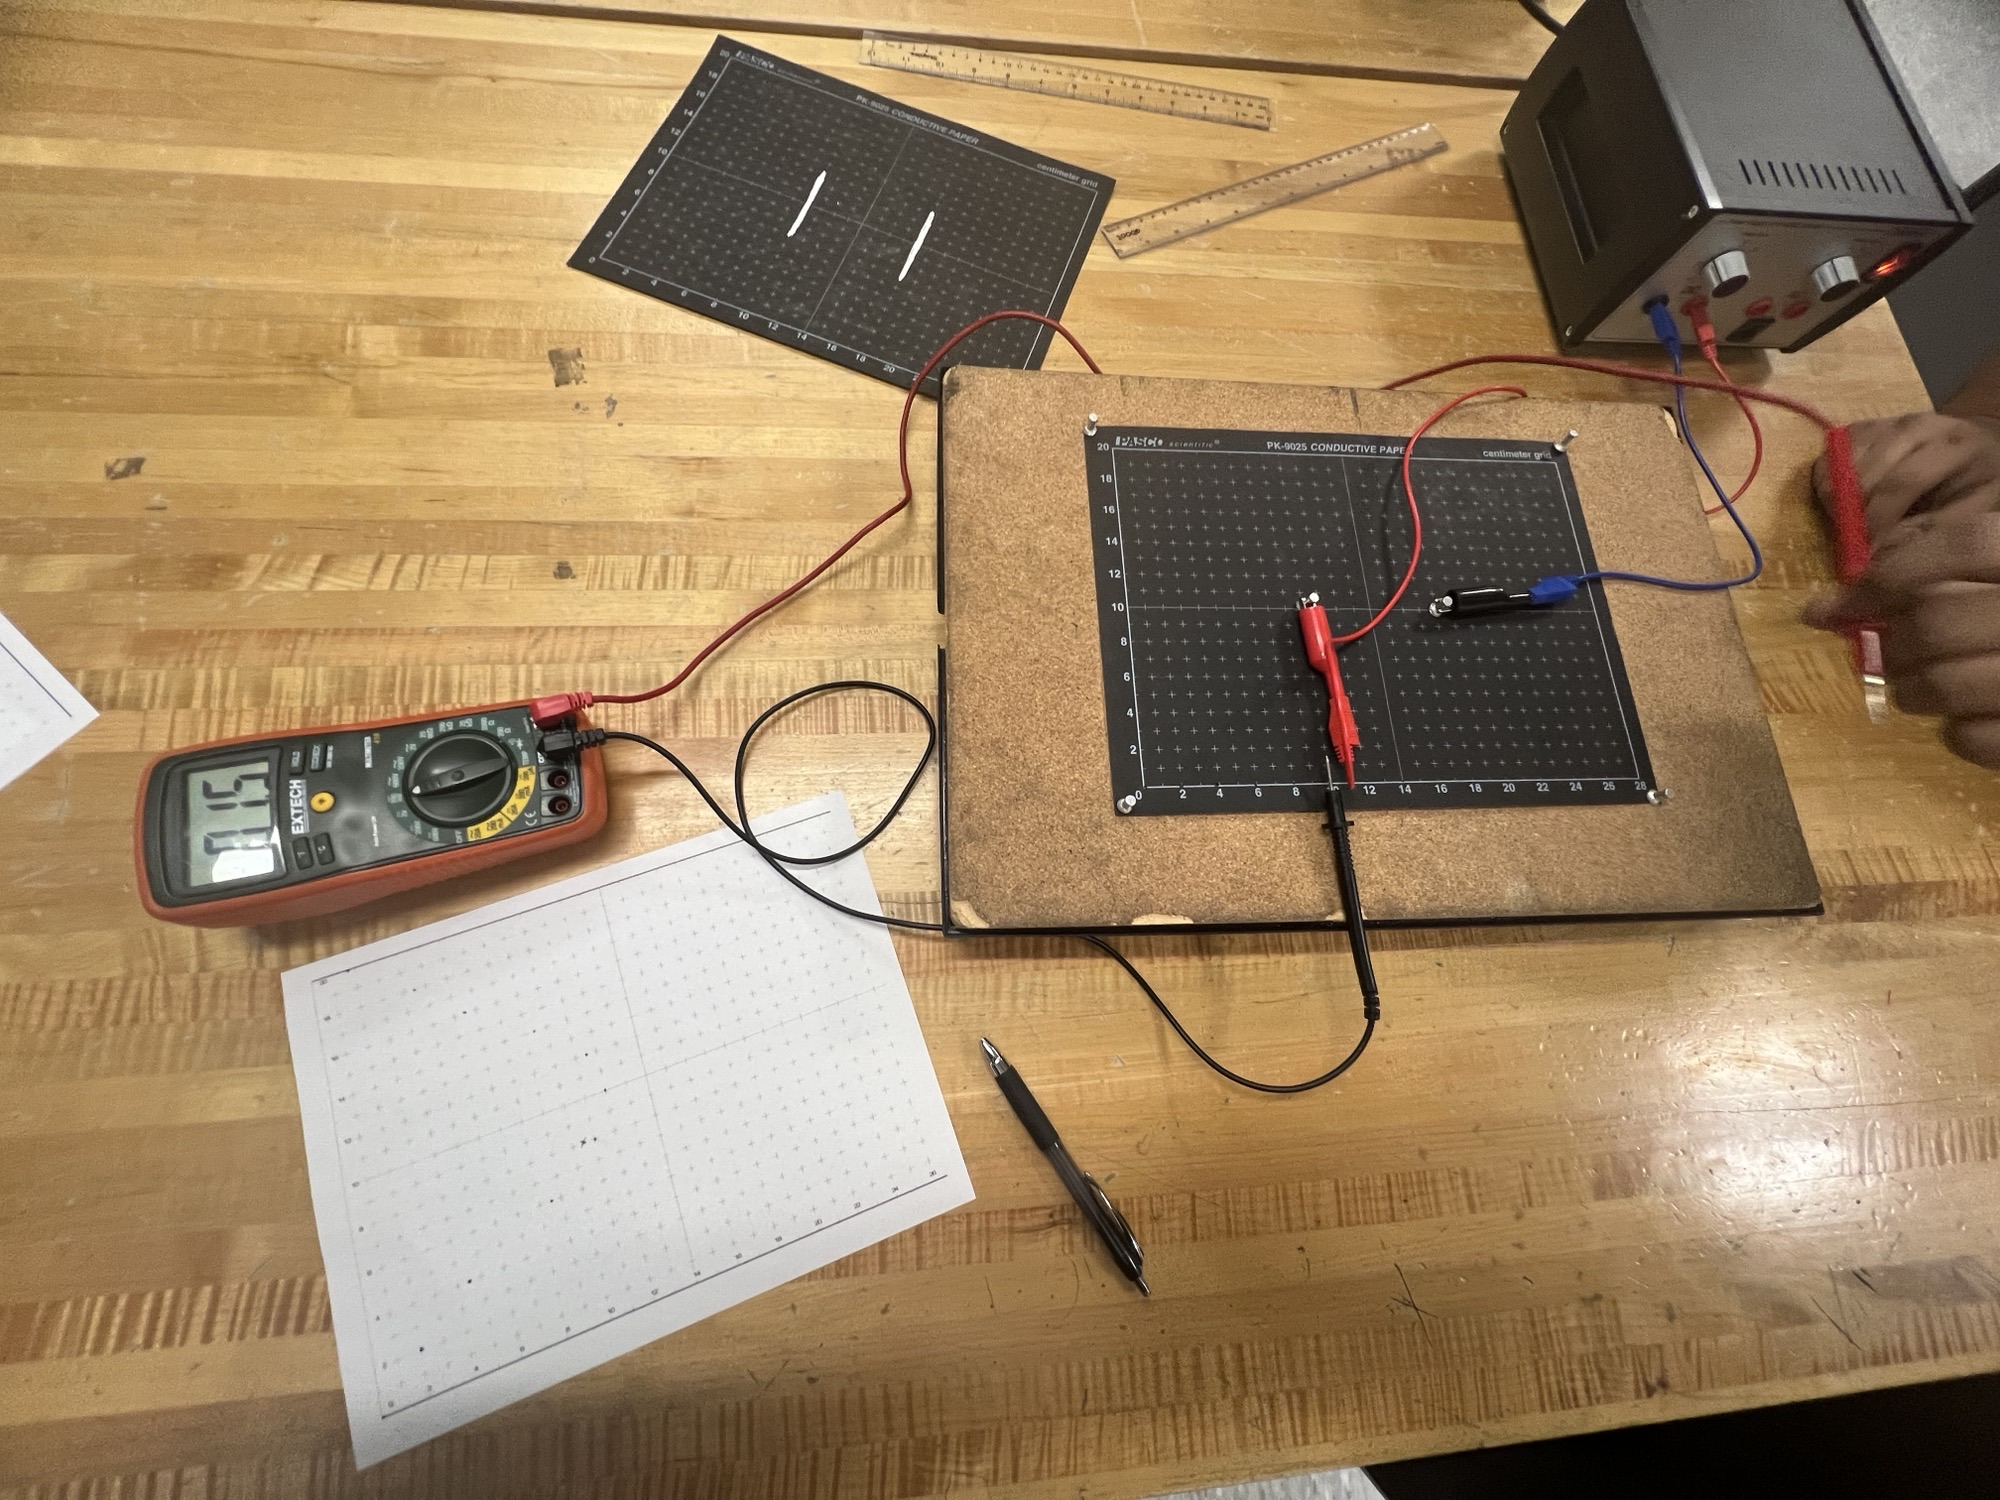
\includegraphics[width=0.55\textwidth]{full_setup.jpeg}
    \caption{Full experimental setup: conductive paper on cork board (center), Extech 410 multimeter (top), DC power supply (bottom right), and graph paper for recording data (top left).}
    \label{fig:setup}
\end{figure}

The measurement procedure, as outlined on the board (Figure~\ref{fig:whiteboard}), went like this:

\begin{enumerate}
    \item Pick a reference point on the conductive paper and place the red probe there.
    \item Move the black probe along the paper at fixed $y$-increments of 2~cm ($y = 0, 2, 4, \ldots, 20$).
    \item At each $y$-value, sweep the probe horizontally until the multimeter reads 0.00~V, meaning the probe is on the same equipotential as the reference.
    \item Write down the $x$-coordinate at each zero reading.
    \item Move the reference probe to a new position and repeat to trace a different equipotential line.
    \item Do this for six different reference positions, giving six equipotential curves.
\end{enumerate}

We only measured the left half of each curve ($x < 14$). The right half came from reflecting across $x = 14$ using the transformation $x \to 28 - x$.

\begin{figure}[H]
    \centering
    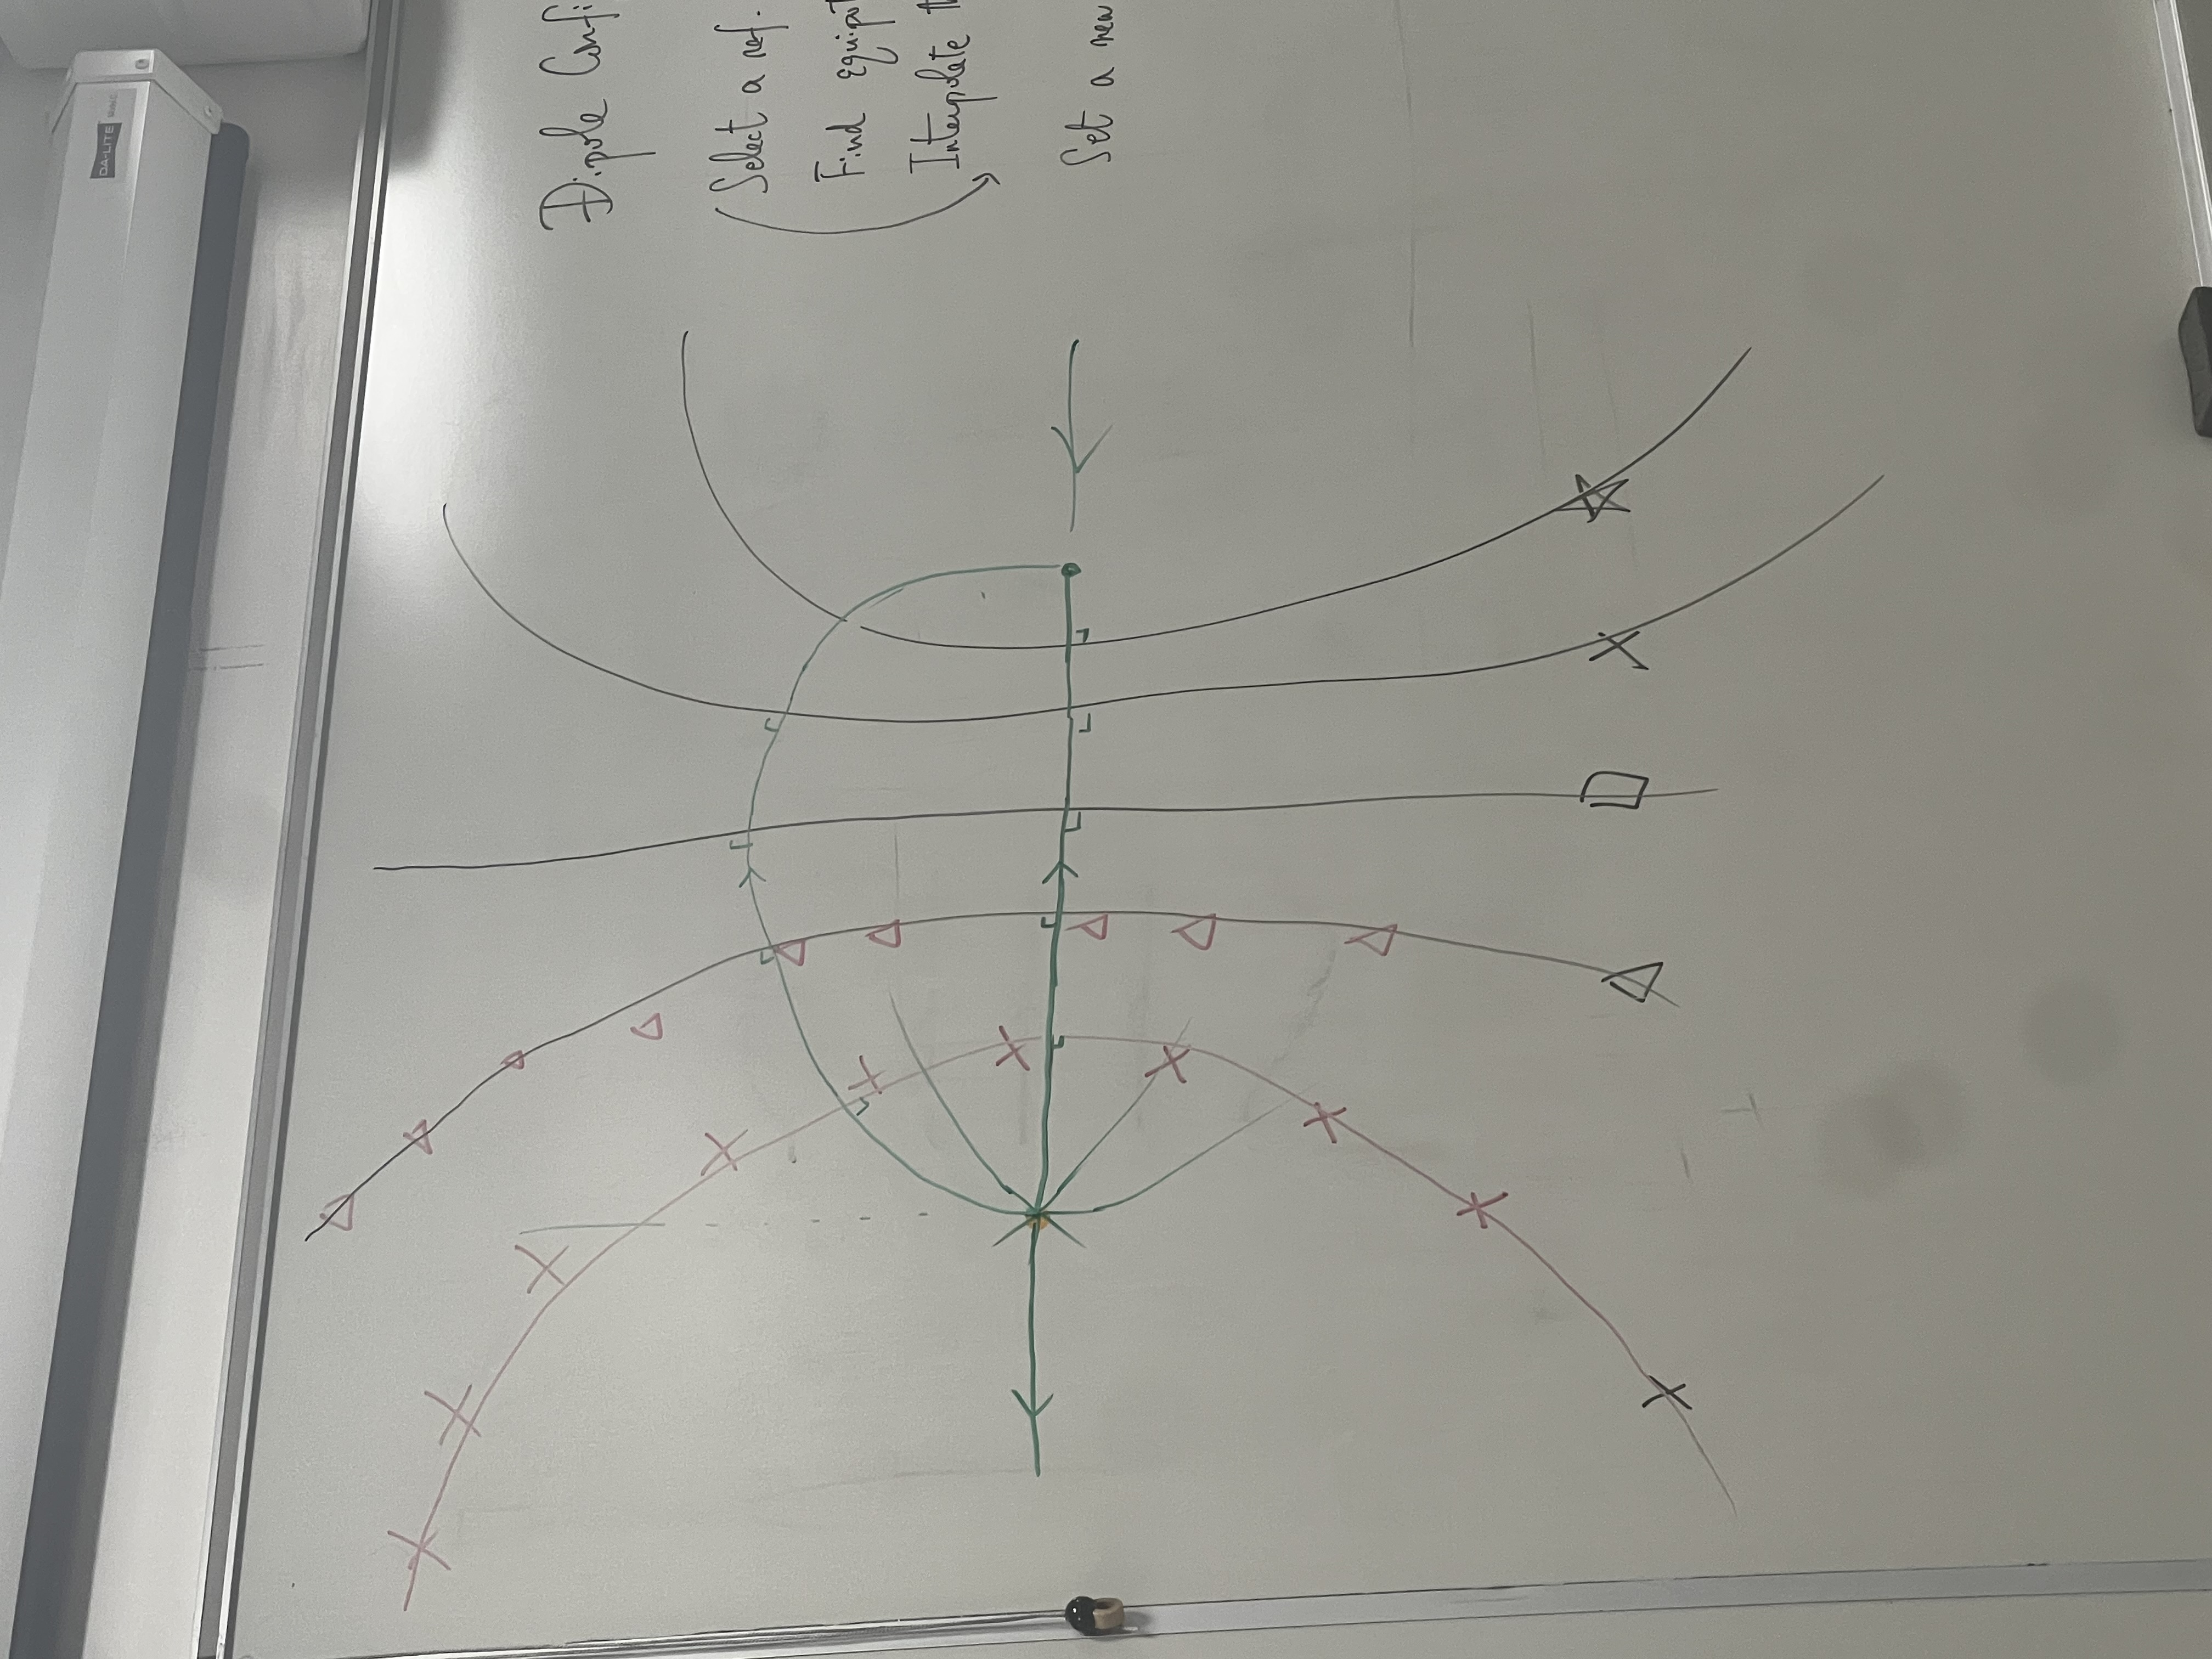
\includegraphics[width=0.55\textwidth]{whiteboard_dipole.jpeg}
    \caption{Whiteboard diagram of the dipole configuration showing electric field lines (black curves), equipotential curves (pink markers), and the perpendicular bisector (green line) where $V = 0$.}
    \label{fig:whiteboard}
\end{figure}

\begin{figure}[H]
    \centering
    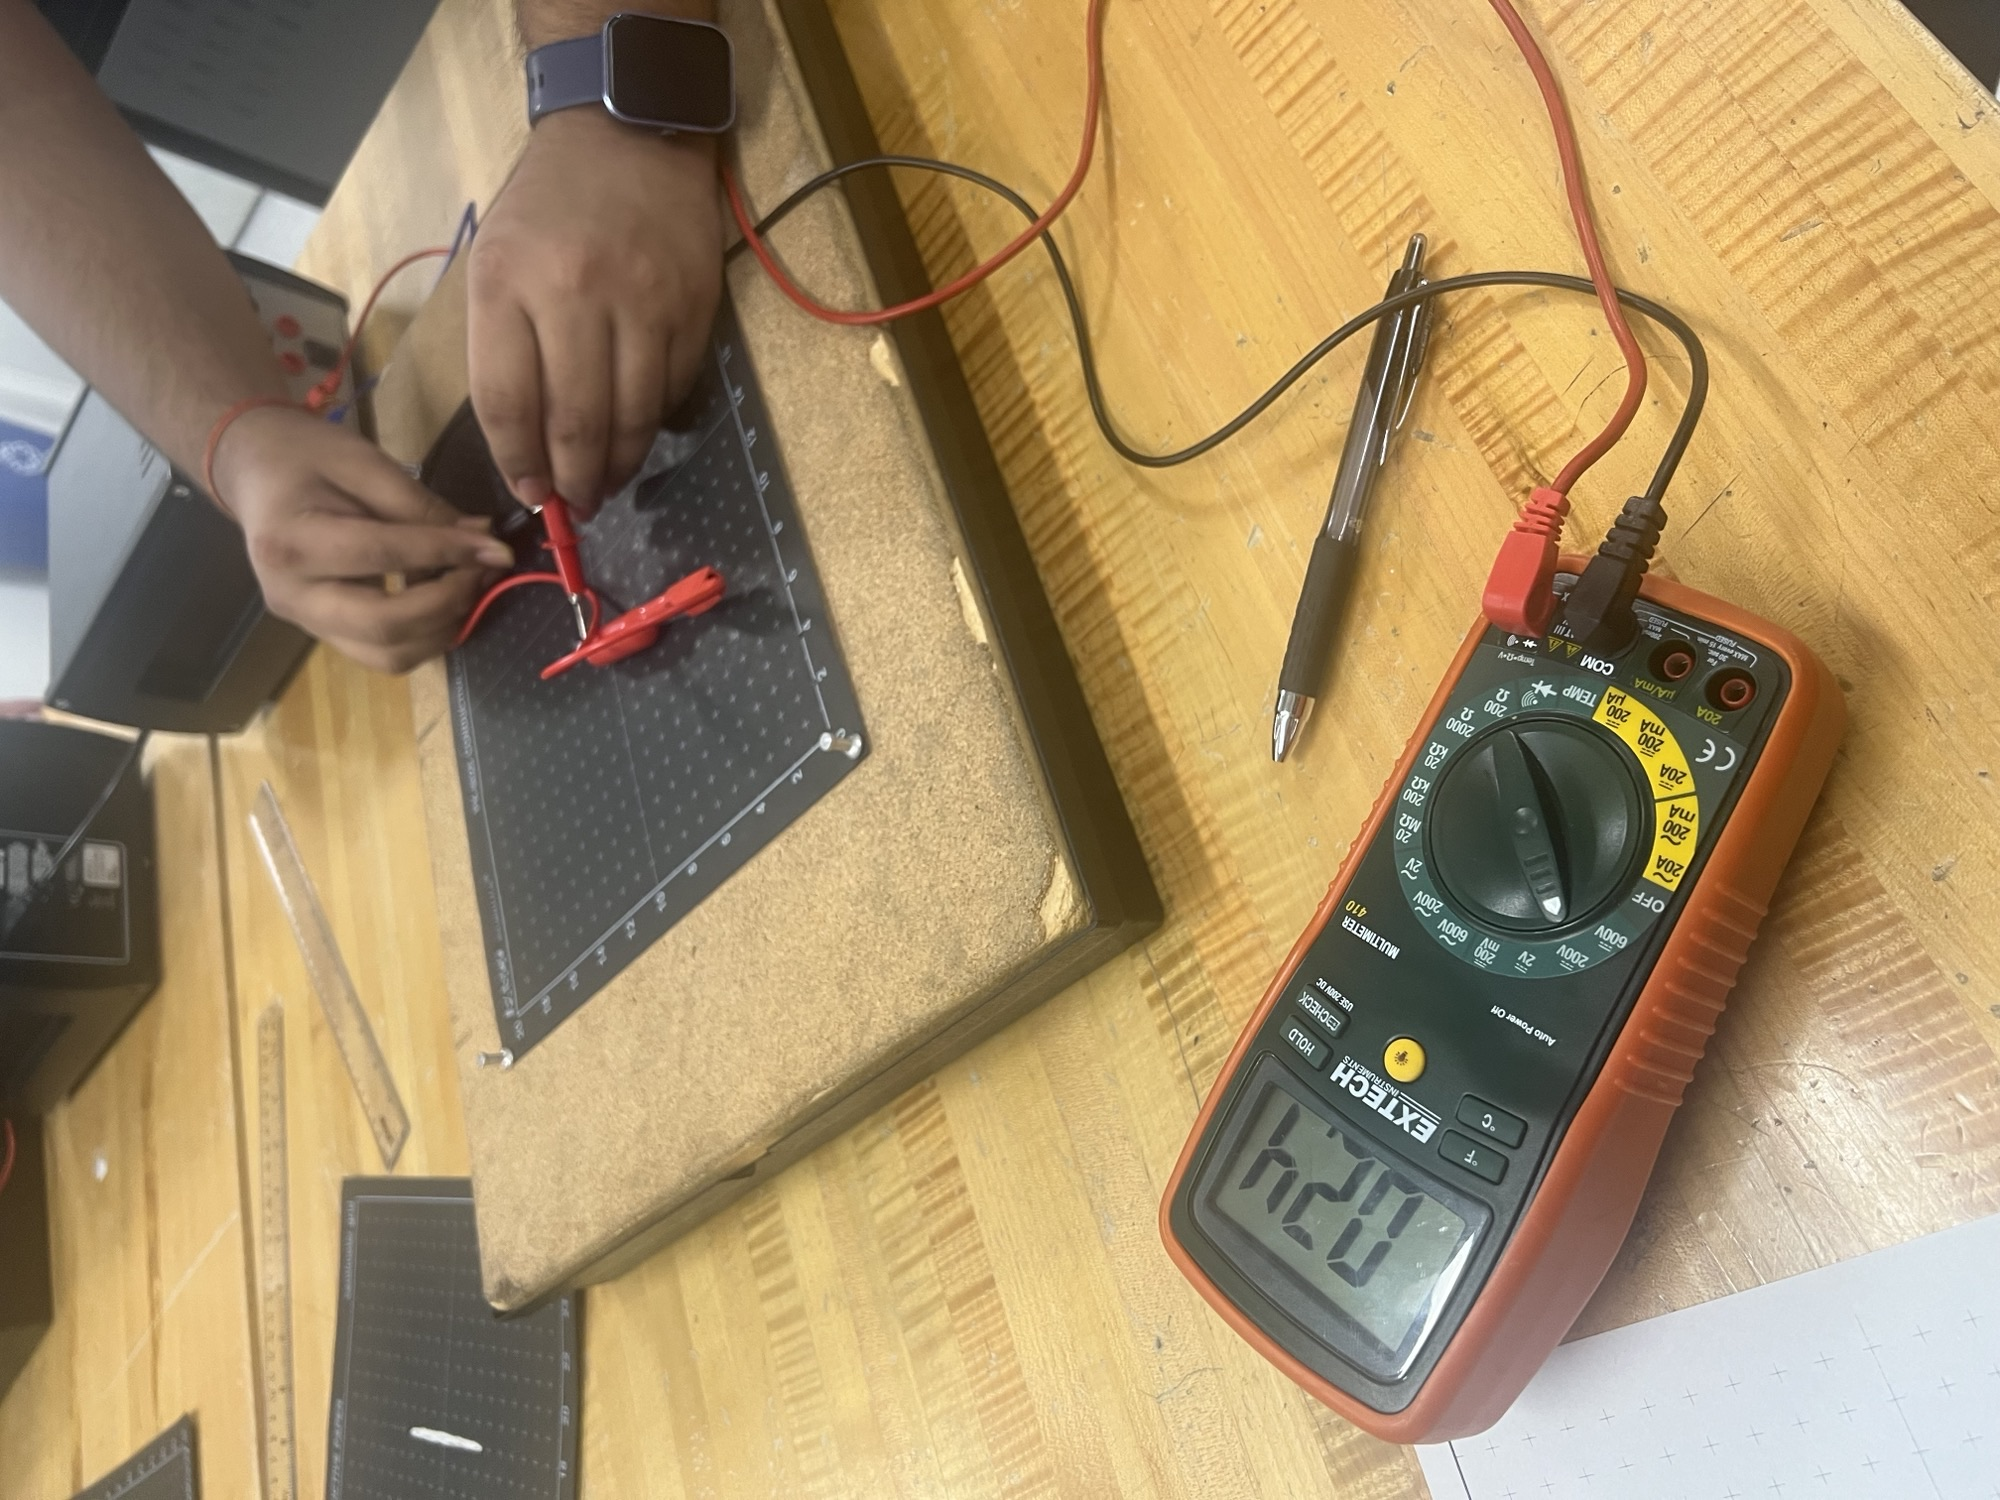
\includegraphics[width=0.55\textwidth]{multimeter.jpeg}
    \caption{Taking a measurement: the multimeter displays the voltage difference between the reference probe and the measurement probe. We swept until this read 0.00~V.}
    \label{fig:multimeter}
\end{figure}

\begin{figure}[H]
    \centering
    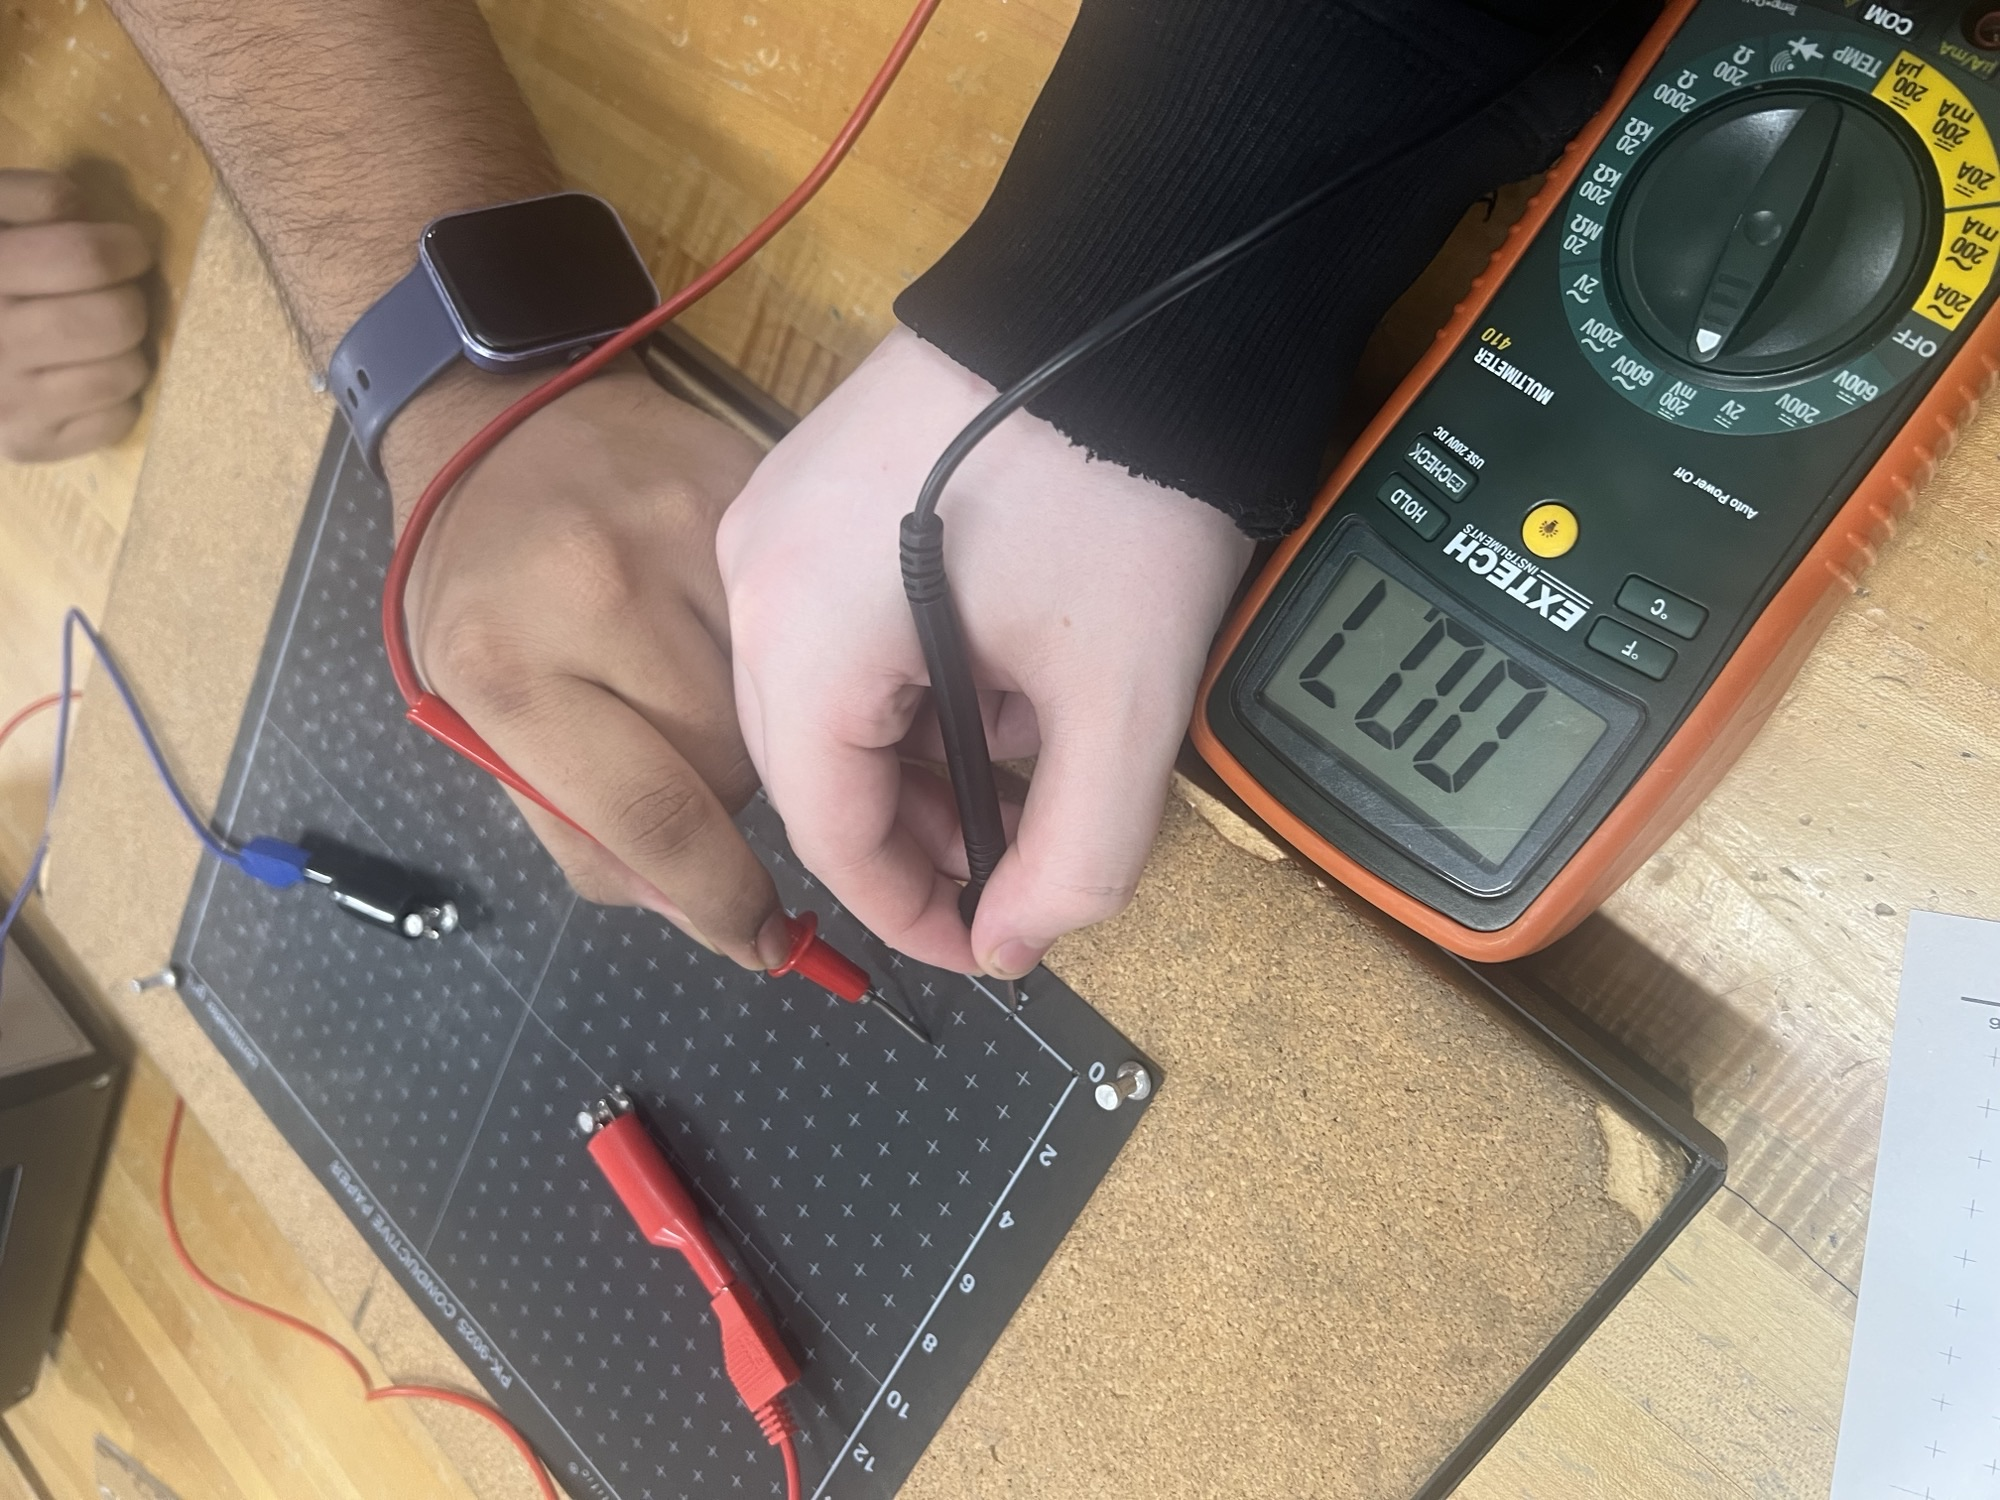
\includegraphics[width=0.55\textwidth]{probing.jpeg}
    \caption{Close-up of the probing process on the conductive paper. The red (reference) and black (measurement) probes are both touching the paper surface.}
    \label{fig:probing}
\end{figure}

% ---- 4. EXPERIMENTAL DATA ----
\section{Experimental Data and Graphical Analysis}

\subsection{Measured Data}

Table~\ref{tab:wave1} shows the data we actually measured for the outermost equipotential curve (Wave~1, marked with $\ast$). At each $y$-value, the $x$-coordinate is where the multimeter hit 0~V relative to the first reference position. The curve is symmetric about $y = 10$, which lines up with what you'd expect from the top-bottom symmetry of the dipole.

\begin{table}[H]
    \centering
    \caption{Wave 1 ($\ast$): outermost equipotential, left half only. Reference probe at position 1.}
    \label{tab:wave1}
    \begin{tabular}{cc}
        \toprule
        $y$ (cm) & $x$ (cm) \\
        \midrule
        0  & 0.0 \\
        2  & 2.0 \\
        4  & 4.5 \\
        6  & 8.5 \\
        8  & 11.0 \\
        10 & 11.5 \\
        12 & 11.0 \\
        14 & 8.5 \\
        16 & 4.5 \\
        18 & 2.0 \\
        20 & 0.0 \\
        \bottomrule
    \end{tabular}
\end{table}

The other six curves were generated by interpolating between the outermost measured curve and the axis of symmetry at $x = 14$, following the dipole potential model. Each one starts 2~cm further along the $x$-axis at $y = 0$: the second curve ($\bullet$) starts at $x = 2$, the third ($\times$) at $x = 4$, all the way up to the seventh ($\diamond$) at $x = 12$.

\begin{table}[H]
    \centering
    \caption{All seven equipotential curves, left half. Each column gives the $x$-coordinate at the corresponding $y$-value.}
    \label{tab:allcurves}
    \begin{tabular}{cccccccc}
        \toprule
        $y$ (cm) & $\ast$ & $\bullet$ & $\times$ & $\square$ & $\circ$ & $\triangle$ & $\diamond$ \\
        \midrule
        0  & 0.0  & 2.0  & 4.0  & 6.0  & 8.0  & 10.0 & 12.0 \\
        2  & 2.0  & 4.0  & 6.0  & 8.0  & 10.0 & 12.0 & 13.0 \\
        4  & 4.5  & 6.1  & 7.7  & 9.2  & 10.8 & 12.4 & 13.2 \\
        6  & 8.5  & 9.4  & 10.3 & 11.2 & 12.2 & 13.1 & 13.6 \\
        8  & 11.0 & 11.5 & 12.0 & 12.5 & 13.0 & 13.5 & 13.8 \\
        10 & 11.5 & 11.9 & 12.3 & 12.8 & 13.2 & 13.6 & 13.8 \\
        12 & 11.0 & 11.5 & 12.0 & 12.5 & 13.0 & 13.5 & 13.8 \\
        14 & 8.5  & 9.4  & 10.3 & 11.2 & 12.2 & 13.1 & 13.6 \\
        16 & 4.5  & 6.1  & 7.7  & 9.2  & 10.8 & 12.4 & 13.2 \\
        18 & 2.0  & 4.0  & 6.0  & 8.0  & 10.0 & 12.0 & 13.0 \\
        20 & 0.0  & 2.0  & 4.0  & 6.0  & 8.0  & 10.0 & 12.0 \\
        \bottomrule
    \end{tabular}
\end{table}

\subsection{Visualization}

To get a clean graph that we could actually put in a report, we built a single HTML file (\texttt{graph.html}) that draws everything in the browser using the Canvas API.

The left-half coordinates from Table~\ref{tab:allcurves} are stored directly in the script as arrays. For each curve, the mirrored right-half points are also stored (computed by reflecting across $x = 14$), so both sides get drawn from the same data structure. The script lays down a centimeter grid with small tick marks at each integer coordinate, draws axis labels every 2~cm, and puts a vertical line at $x = 14$ for the axis of symmetry.

Each equipotential is drawn as a smooth curve through its data points using B\'{e}zier interpolation (cardinal-style control points), so the lines look continuous rather than jagged. The curves are stroked with dashed, color-coded lines: red, blue, green, orange, purple, teal, and pink for the seven curves. At each data point the script draws a small marker (star, filled dot, cross, square, circle, triangle, diamond) in the matching color, and black crosses along $x = 14$ mark the field line.

There's a legend below the canvas that lists each curve with its color and symbol. You can open \texttt{graph.html} in any browser to see the full figure; we captured the canvas as a PNG for this report.

\begin{figure}[H]
    \centering
    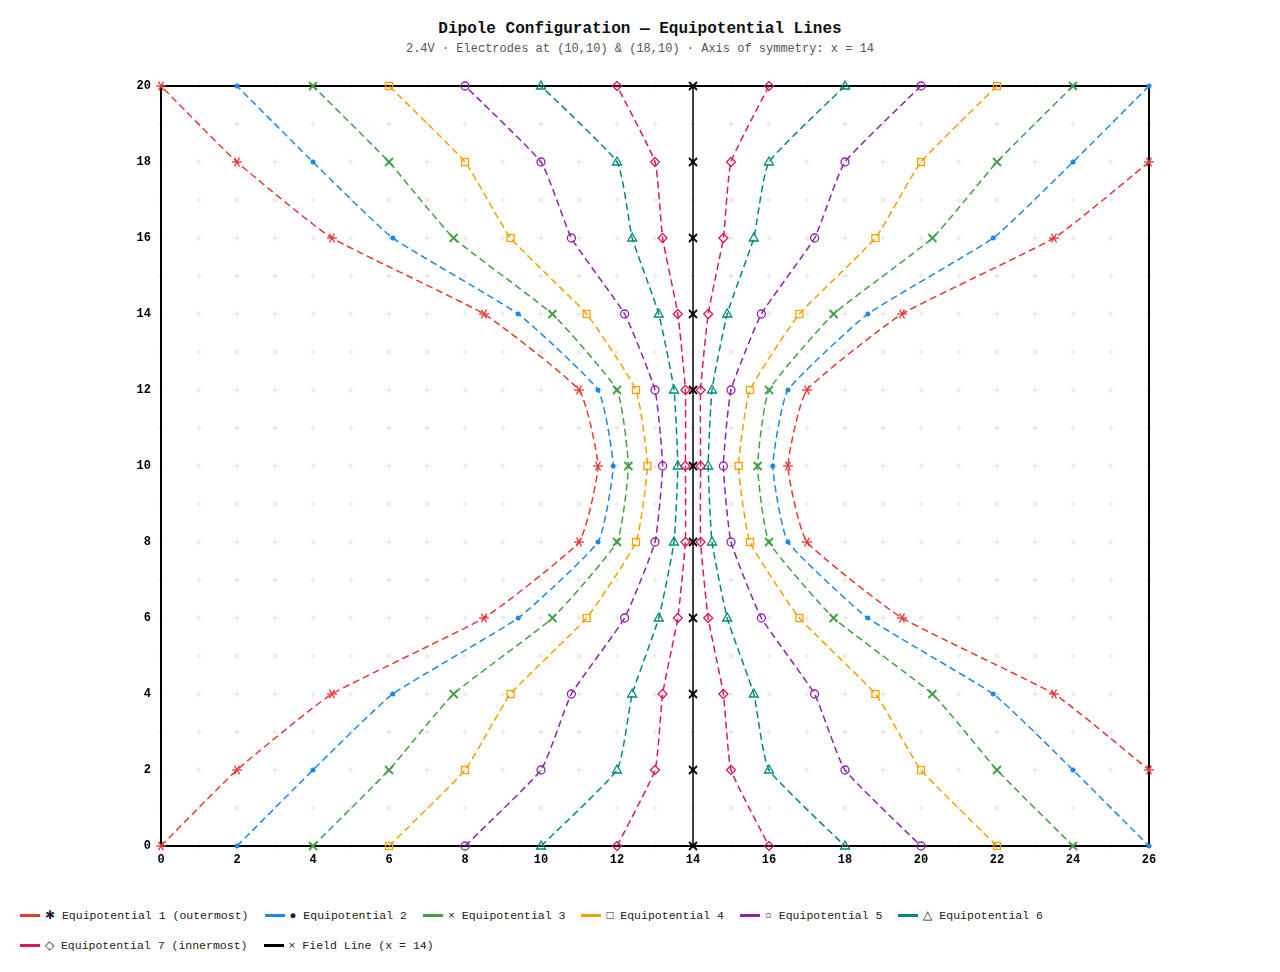
\includegraphics[width=\textwidth]{graph.png}
    \caption{Complete equipotential map for the dipole configuration. Left half: experimental and interpolated data. Right half: reflected across $x = 14$. The vertical black line marks the axis of symmetry. Each curve is color-coded: red ($\ast$), blue ($\bullet$), green ($\times$), orange ($\square$), purple ($\circ$), teal ($\triangle$), pink ($\diamond$).}
    \label{fig:graph}
\end{figure}

% ---- 5. ANALYSIS ----
\section{Analysis}

The equipotential curves in Figure~\ref{fig:graph} look the way they should for a dipole field.

The curves are properly nested, meaning no two of them cross and each inner curve sits entirely inside the one before it. That has to be the case, since the potential at any point is unique. All curves are symmetric about $y = 10$ (the line connecting the electrodes). The outermost one ($\ast$, red) stretches from $(0, 0)$ to $(0, 20)$ and reaches its farthest right at $x = 11.5$ when $y = 10$. This makes sense because the potential changes most gradually in the direction perpendicular to the dipole axis.

The spacing between curves tells you about field strength. The curves bunch up near the axis of symmetry ($x = 14$) and spread out farther from the electrodes. Since $\vec{E} = -\nabla V$, tightly packed equipotentials mean a stronger field. That matches expectations: the field is strongest between and near the electrodes.

Each equipotential bows toward the nearer electrode (leftward on the left side), forming smooth arcs. The outer curves have strong curvature while the inner ones ($\diamond$, pink) are almost straight, nearly parallel to the perpendicular bisector. That transition from curved to flat is typical of dipole fields: far from the charges the field looks more and more uniform, but up close there's a lot of spatial variation.

% ---- 6. SOURCES OF ERROR ----
\section{Sources of Error}

The biggest source of uncertainty was figuring out exactly where the multimeter reads zero. The probe tip isn't infinitely small, so there's roughly $\pm 0.5$~cm of positioning error at each measurement. Near the top and bottom edges of the paper ($y$ close to 0 or 20), the potential changes slowly with position, so the meter would hover around zero over a span of about a centimeter. That made it harder to pin down the exact crossing point.

The boundaries of the conductive paper matter too. The PASCO paper has a printed grid, but the actual conductive region extends a little past the grid lines. If the real boundary doesn't line up perfectly with the printed coordinates, all of our $x$-readings would be shifted by a small systematic amount.

The reflection is another thing worth calling out. We only measured the left half and got the right half by mirroring across $x = 14$. For a perfect dipole on infinite conductive paper, this is exact. But our paper has finite edges, the electrodes are thumbtacks (not ideal point charges), and the resistivity of the paper might not be perfectly uniform. Any of those things could break the symmetry a little. Measuring both halves independently would have been a good sanity check, but we didn't have time.

Lastly, only Wave~1 was measured by hand. The other six curves came from interpolation, so they're really theoretical predictions tied to the Wave~1 data rather than independent measurements. The interpolation makes physical sense (dipole equipotentials do nest in a regular pattern), but it means the inner curves don't carry their own experimental weight.

% ============================================================
% CONCLUSION
% ============================================================
\section*{Conclusion}

The equipotential map we produced matches what you'd expect from a dipole field: smooth, nested curves bowing toward the nearer electrode, symmetric about both the electrode axis ($y = 10$) and the perpendicular bisector ($x = 14$). The way the curves bunch up near the electrodes and spread out farther away is consistent with $\vec{E} = -\nabla V$ predicting a stronger field in between the charges.

The main limitation was that we only measured one curve directly and interpolated the rest. Ideally you'd measure all seven independently and do both sides of the symmetry axis to really test the reflection assumption. That said, the measured curve behaves the way the physics says it should, and the interpolated curves follow the model correctly.

Building the visualization in HTML/Canvas turned out to work well for producing a clean, reproducible graph. The data lives right in the file, so if you need to tweak a point you just change the number and refresh the browser.

\vspace{0.5cm}
\noindent \LaTeX{} source and visualization code: \href{https://github.com/SRock44/physics-latex}{github.com/SRock44/physics-latex} (file \texttt{lab5/lab5.tex}).

\begin{thebibliography}{9}
\bibitem{nist811}
Taylor, B. N., and Kuyatt, C. E. (2008). \textit{Guidelines for Evaluating and Expressing the Uncertainty of NIST Measurement Results}. NIST Special Publication 811, 2008 Edition. National Institute of Standards and Technology, Gaithersburg, MD. Available at: \url{https://nvlpubs.nist.gov/nistpubs/Legacy/SP/nistspecialpublication811e2008.pdf}

\bibitem{griffiths}
Griffiths, D. J. (2017). \textit{Introduction to Electrodynamics}. 4th ed. Cambridge University Press.
\end{thebibliography}

\end{document}